\chapter{Requirements Specification and Project Schedule}

\theoremstyle{plain}
\theoremsymbol{}
\newtheorem{Rule}[theorem]{Rule}

\pagebreak
\section{Requirements Specification}

\begin{figure}[h!]
    \centering
	\frame{
\includegraphics[width=14.45cm, page=1]{appendix/Requirements_Specification}}
\end{figure}
\pagebreak

\begin{figure}[h!]
	\centering
	\vspace{1.4cm}
	\frame{
\includegraphics[width=14.45cm, page=2]{appendix/Requirements_Specification}}
\end{figure}
\pagebreak

\begin{figure}[h!]
	\centering
	\vspace{1.4cm}
	\frame{
\includegraphics[width=14.45cm, page=3]{appendix/Requirements_Specification}}
\end{figure}
\pagebreak

\begin{figure}[h!]
	\centering
	\vspace{1.4cm}
	\frame{
\includegraphics[width=14.45cm, page=4]{appendix/Requirements_Specification}}
\end{figure}
\pagebreak

\begin{figure}[h!]
	\centering
	\vspace{1.4cm}
	\frame{
\includegraphics[width=14.45cm, page=5]{appendix/Requirements_Specification}}
\end{figure}
\pagebreak

\begin{figure}[h!]
	\centering
	\vspace{1.4cm}
	\frame{
\includegraphics[width=14.45cm, page=6]{appendix/Requirements_Specification}}
\end{figure}
\pagebreak

\begin{figure}[h!]
	\centering
	\vspace{1.4cm}
	\frame{
\includegraphics[width=14.45cm, page=7]{appendix/Requirements_Specification}}
\end{figure}
\pagebreak



\begin{landscape}
    \section{Project Schedule}
    \begin{figure}[h!]
    	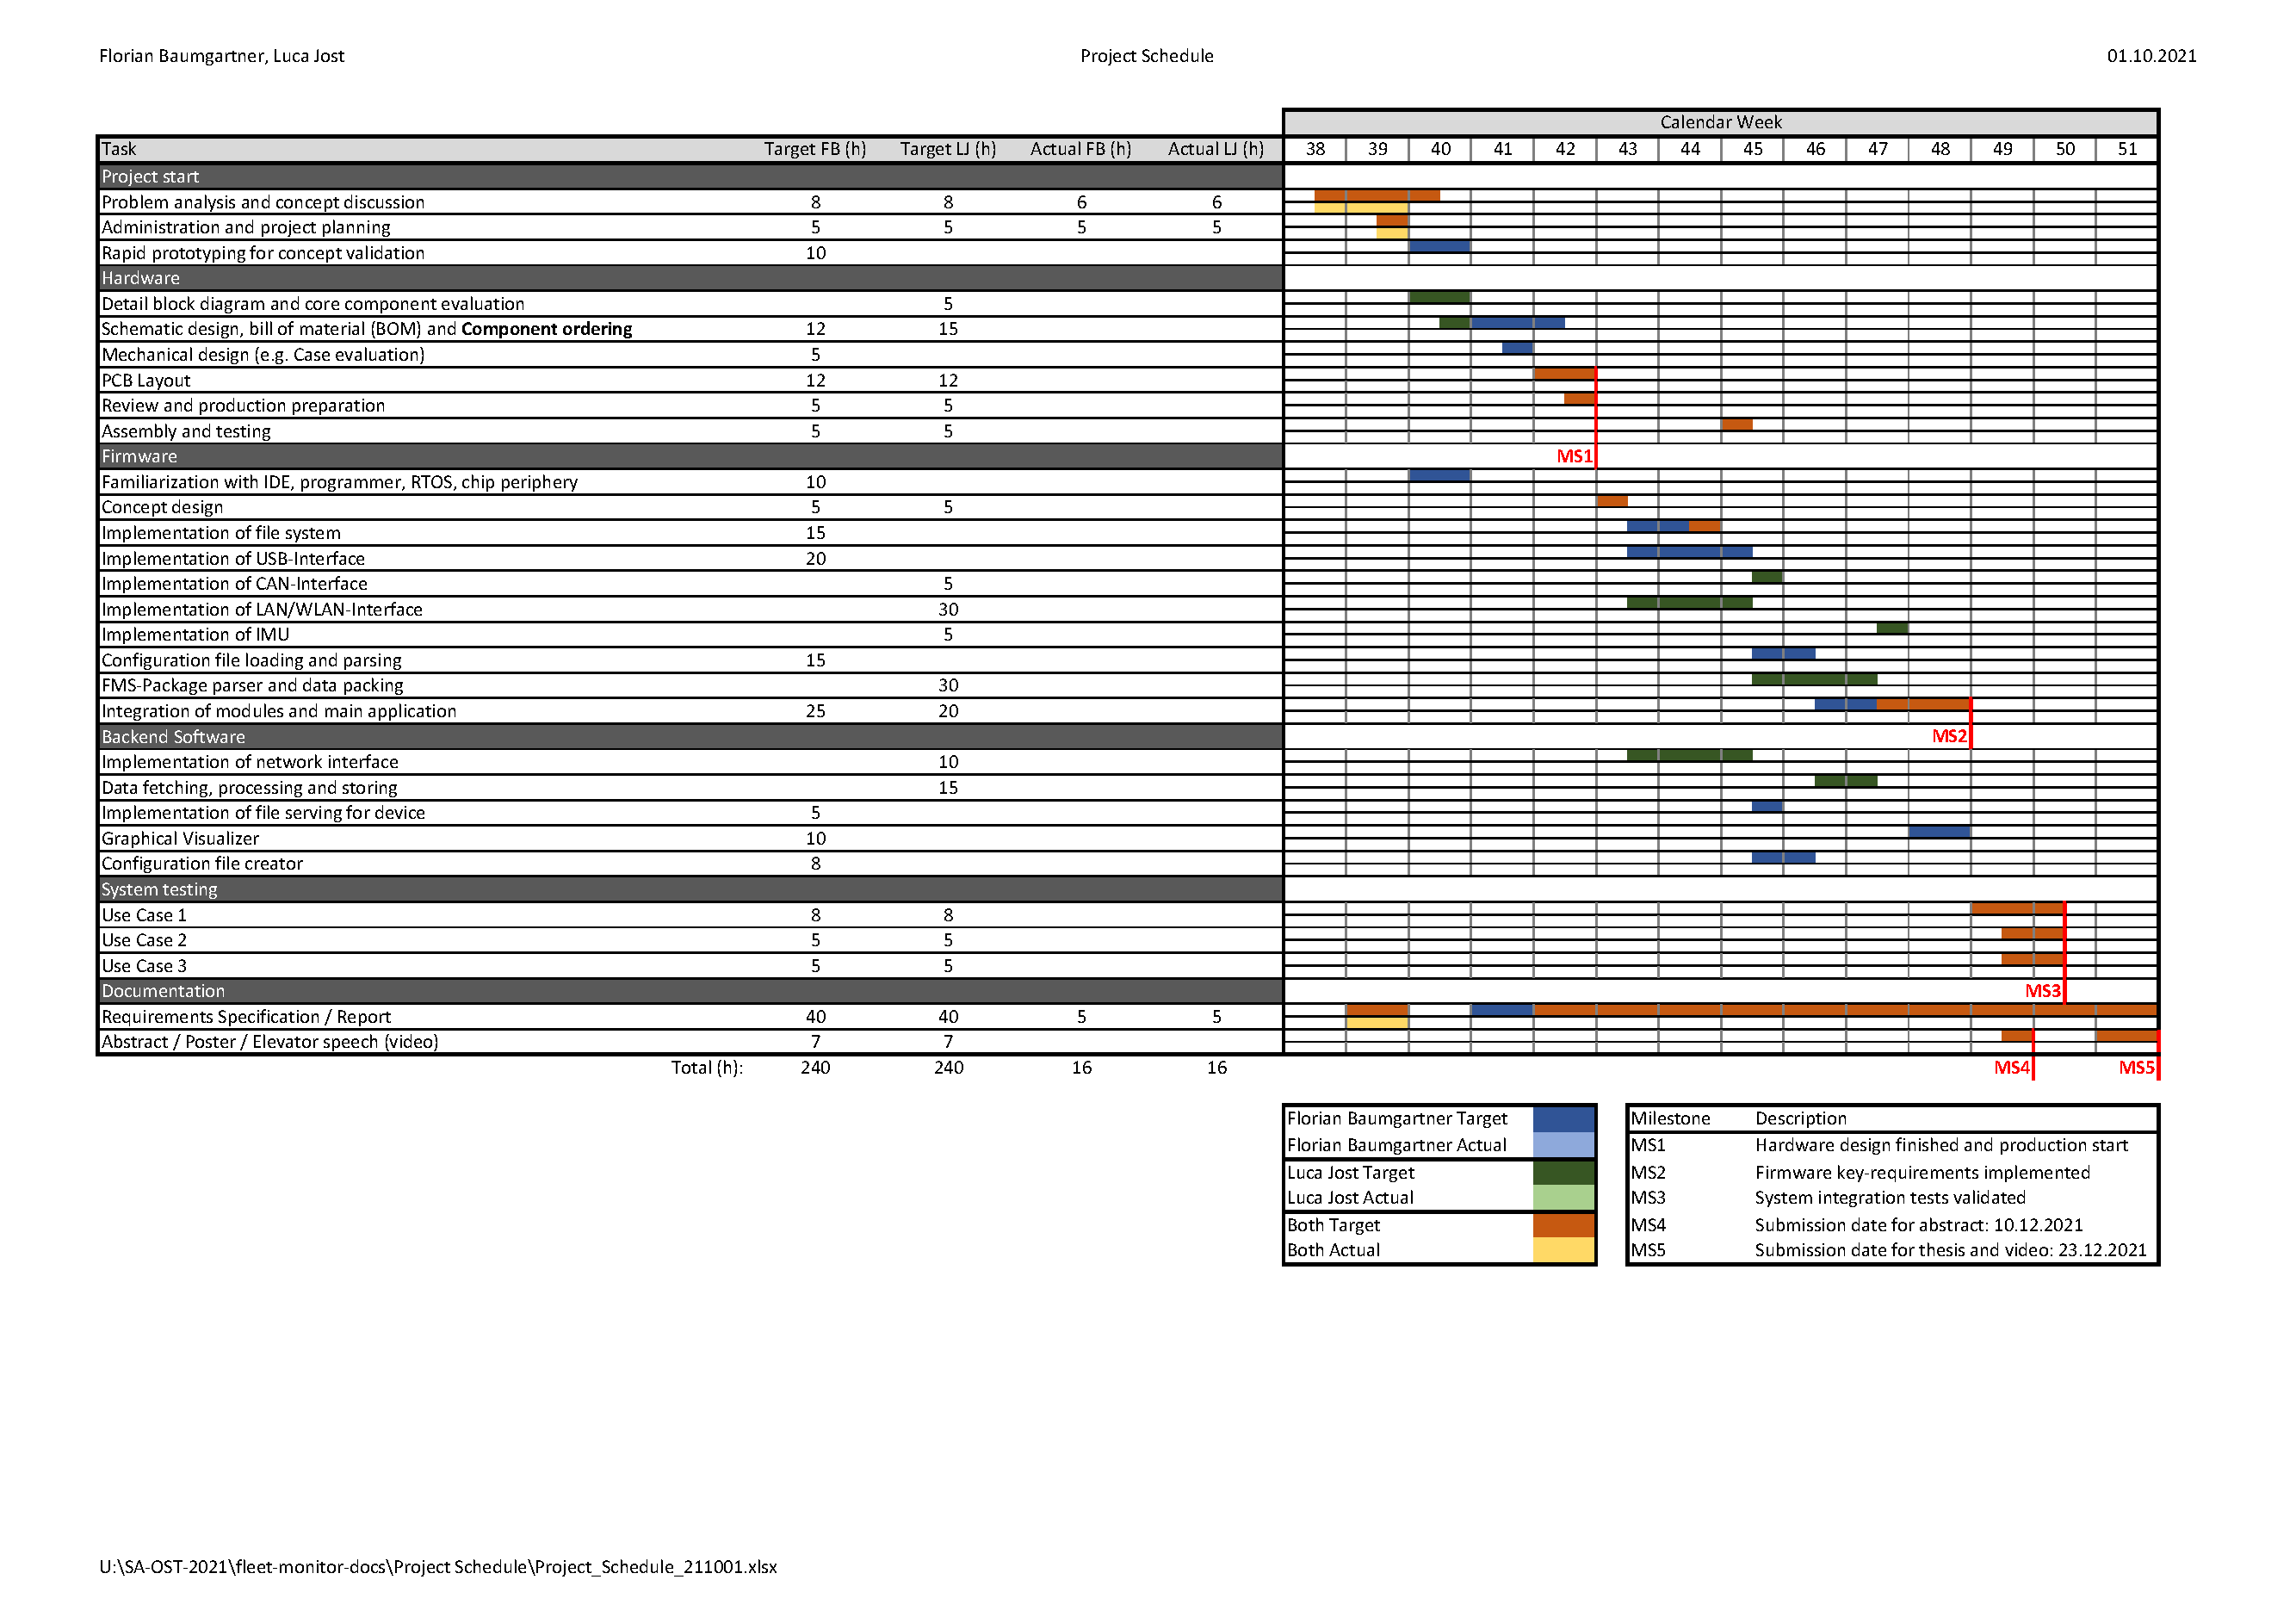
\includegraphics[height=13cm, trim=17mm 69mm 25mm 20mm, clip]{appendix/Project_Schedule_211001}
    	\bigskip
    	\caption{Project Schedule}
	    \vspace{-2cm}
	    \label{fig:project_schedule}
    \end{figure}
    \pagebreak

\end{landscape}